% =============================================================================
% CHAPTER 2: DATA ANALYSIS PROJECT (Major competency 1)
% =============================================================================
% Replace "PROJECT TITLE 1" with your project title.
% See INSTRUCTIONS.md for how to add figures, tables, citations, abbreviations.
% =============================================================================

\chapter{PROJECT TITLE 1}
\label{chap:project_1}
\clearpage

\setcounter{tocdepth}{5}
\setcounter{secnumdepth}{4}
\etocdepthtag.toc{mtchapter}

\localtoc
\clearpage

% LOCAL LIST OF TABLES — remove this line if this chapter has no tables
\locallistoftables
% LOCAL LIST OF FIGURES — remove this line if this chapter has no figures
\locallistoffigures
\clearpage

\glsresetall[abbreviations]


% =============================================================================
\section{Prologue}
% =============================================================================

\subsection{Study rationale}

\subsection{My role}

\subsection{Lessons learnt}

\subsection{Public health impact}

\subsection{MAE competencies addressed}
\begin{itemize}
  \item Analysis of a public health dataset
  \item Report to a non-scientific audience
\end{itemize}

\subsection{Acknowledgements}


% =============================================================================
% Abbreviations reset here so they expand in full within the Abstract.
\glsresetall[abbreviations]
\clearpage
\section{Abstract}
% =============================================================================


% =============================================================================
% Abbreviations reset again so they expand in full in the main body.
\glsresetall[abbreviations]
\clearpage
\section{Introduction}
% =============================================================================
The is an example of a reference \cite{national_health_and_medical_research_council_nhmrc_2015}.

% =============================================================================
\section{Methods}
% =============================================================================

\subsection{Study period and population}

\subsubsection{Surveillance case definition}

\subsection{Data collection}
\gls{EHU} conducted field investigations and interviewed cases. \gls{EHU} upload the data collected during these investigations to \gls{REDCap}.

\subsection{Data cleaning}

\subsection{Data analysis}

\subsection{Ethics}


% =============================================================================
\section{Results}
% =============================================================================
% Reference every figure and table in the text before it appears.
%
% HOW TO ADD A TABLE (save image to data_analysis/tables/):
%
%   \begin{table}[H]
%       \caption{Caption goes ABOVE the table.}
%       \label{tab:my_table}
%       \centering
%       \begin{tabular}{c}
%           \includegraphics[width=0.95\textwidth]{data_analysis/tables/my_table.png}
%       \end{tabular}
%   \end{table}
%   Reference in text: \cref{tab:my_table}  →  "Table 1"
%
% HOW TO ADD A FIGURE (save image to data_analysis/figures/):
%
%   \begin{figure}[H]
%       \centering
%       \includegraphics[width=0.85\textwidth]{data_analysis/figures/my_figure.png}
%       \caption{Caption goes BELOW the figure.}
%       \label{fig:my_figure}
%   \end{figure}
%   Reference in text: \cref{fig:my_figure}  →  "Figure 1"

\begin{table}[H]
    \caption{Number of cases by age group (not real data).}
    \label{tab:age_table}
    \centering
    \begin{tabular}{c}
        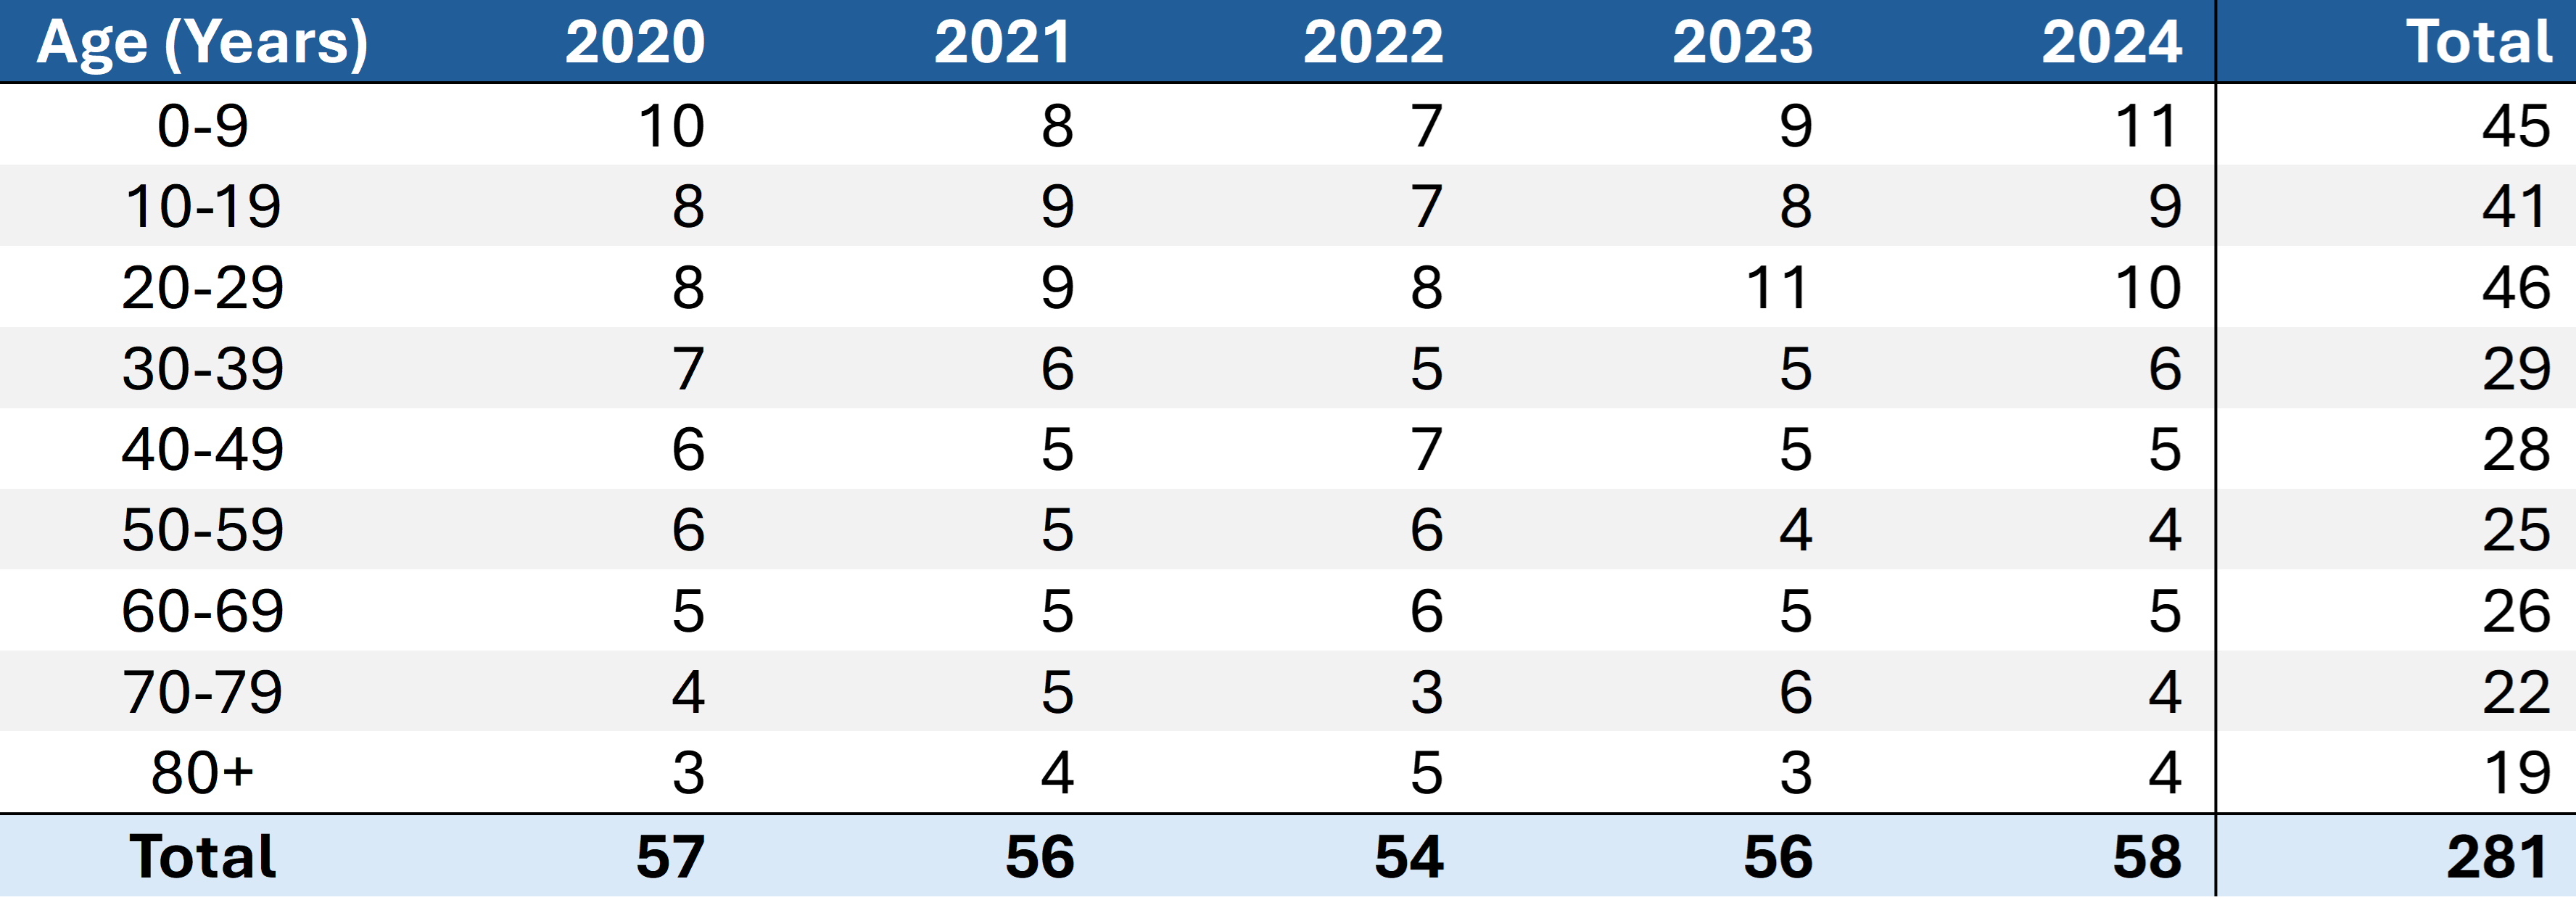
\includegraphics[width=0.95\textwidth]{data_analysis/tables/age_table_example.png}
    \end{tabular}
\end{table}


% =============================================================================
\section{Discussion}
% =============================================================================


% =============================================================================
\section{Limitations}
% =============================================================================


% =============================================================================
\section{Conclusion}
% =============================================================================


% =============================================================================
\clearpage
\section{Recommendations}
% =============================================================================

% Each recommendation should name the responsible party in bold italics.
\textit{\textbf{Responsible: [Unit/team name]}}

Recommendation text here.


% =============================================================================
% REFERENCES — do not edit these two lines
% =============================================================================
\clearpage
\addcontentsline{toc}{section}{References}
\printbibliography[heading=subbibliography, title={References}]


% =============================================================================
% APPENDICES
% Uncomment the section(s) relevant to this chapter.
% Upload your files to data_analysis/appendices/ before including them.
% REMOVE the entire subappendices block if this chapter has no appendices.
% =============================================================================
\begin{subappendices}

% HOW TO INCLUDE A PDF APPENDIX
% Each page of your PDF is included as a separate \includegraphics line.
% Add or remove \includegraphics lines to match the number of pages in your file.
% Upload your PDF to the data_analysis/appendices/ folder before compiling.
% Tip: avoid spaces in filenames — use underscores instead (e.g. my_factsheet.pdf).

% --- LAY SUMMARY / FACTSHEET ---
\clearpage
\section{Lay summary}
\label{app:lay_summary}
\nopagebreak
\centering

\includegraphics[page=1, width=\textwidth]{data_analysis/appendices/factsheet.pdf}
% Add more \includegraphics lines here for additional pages
\RaggedRight

% --- CONFERENCE PRESENTATION SLIDES ---
% \clearpage
% \section{Conference presentation slides}
% \label{app:presentation}
% \nopagebreak
% \centering
% \includegraphics[page=1,width=\textwidth]{data_analysis/appendices/presentation.pdf}
% \clearpage
% \includegraphics[page=2,width=\textwidth]{data_analysis/appendices/presentation.pdf}
% % Add more \includegraphics lines here for additional pages
% \RaggedRight

% --- MANUSCRIPT ---
% \clearpage
% \section{Manuscript}
% \label{app:manuscript}
% \nopagebreak
% \centering
% \includegraphics[page=1,width=\textwidth]{data_analysis/appendices/manuscript.pdf}
% \clearpage
% \includegraphics[page=2,width=\textwidth]{data_analysis/appendices/manuscript.pdf}
% % Add more \includegraphics lines here for additional pages
% \RaggedRight

\end{subappendices}
